
\begin{abstract}

\end{abstract}
\section{Introduction}
Internet privacy, also commonly referred to as online privacy, is a subset of data privacy and a fundamental human right. We consider privacy to revolve around control, use and disclosure of one’s personally identifiable information.
However, our increasingly technologically-driven world puts great pressure on privacy. 
This is why several actors in the space are continuesly developinng different solutions to achieve anonymous communication and thus leveraging internet privacy.


\subsection{State of the art}
\subsubsection{Privacy protocols}
VPN or Virtual Private Network is a privacy technology that allows creating a secure connection on the internet by building an encrypted tunnel between the client and server. VPN also provides a new IP address (the one of the proxy) to help bypass censership and geolocalization blocks.
Due to the centralized trust model VPNs has, they suffer from inherent weaknesses like being a single point of failure. They are also vulnerable to powerful network eavedropers who can track the routed network traffic.
\\Those privacy concerns have motivated the creation of a new model of VPNs, dVPNs (Decentralized Virtual Private Networks) with no central authority and backed by blockchain technology. Orchid, Sentinel and Mysterium are the most known projects in the blockchain ecosystem providing dVPN solutions. These projects however lack privacy, performance and reliability guarantees due to the fact that regular internet users can be both bandwidth providers and normal users. One of the main reasons behind using decentralized VPN instead of a centralized one is to implement a no traffic logging policy as a way to increase privacy, this however introduces the risk of using the service illegally (terrorism, drug smugling, child pornography...etc) which holds service providers reliable to government authorities without them having any legal protection as large VPN providers would have. There have also been some incidents reported, where unaware dVPN users have been (ab)used as exit nodes through which DDoS attacks were performed. Similarly to VPN, users have no guarantee whether a dVPN might inspect, log, and share any of their traffic. A promising project called VPN$^0$ started by the Brave team which provides better privacy guarantees by leveraging zero knowledge proofs to hide traffic content to relay nodes with traffic accounting and traffic blaming capabilities as a way to combat the weaknesses of other dVPN solutions. This project is still research oriented though.
\\~\\ Another existing solution for network privacy is Tor, an open-source software for enabling anonymous communication. Tor is based on onion routing which encapsulates messages in layers of encryption and transmits them through a series of network nodes called onion routers. Tor however is susceptible to end-to-end correlation attacks conducted by an adversary who can eavesdrop the communication channels.These attacks reveal a wide range of information like the identity of the communicating peers.
Another project based on onion routing is I2P peer-to-peer network. I2P has different design choices from those of Tor:
\begin{itemize}
    \item Packet switched instead of circuit switched: Tor allocates connection to long lived circuits, this allocation does not change until either the connection or circuit closes. On the other hand, routers in I2P maintain multiple tunnels per destination which increases significantly the scalability and resilience against failures since packets are used in parallel.
    \item Unidirectional instead of bidirectional tunnels: which makes deanonymization harder since tunnel participants see half as much data in unidirectional tunnels and need two sets of peers to be profiled.
    \item Peer profiles instead of directory authorities: I2P’s network information is stored in a DHT (information in the DHT is inherently untrusted) while Tor’s relay network is managed by a set of nine Directory Authorities.

\end{itemize}
I2P are vulnerable to eclipse attacks since no I2P router has a full view of the global network (similar to other peer-to-peer networks) and they also protect against only local adversaries (like Tor) and thus vulnerable to timing, intersection and traffic analysis attacks. I2P have also showed to be vulnerable to sybil and predecessor attacks inspite of the different contermeasures implemented to defeat them.
\\~\\Mixnets are overlay networks of mix nodes that route messages anonymously similarly to Tor. First mixnet paper in 1981 by David Chaum used a cascade topology where each node receives a batch of encrypted messages, decrypts, randomly permutes packets, and transfers them in parallel. Cascade topology makes it easy to prove the anonymity properties of a given mixnet design for a particular mix, however, it does not scale well with respect to increasing mixnet traffic and is also susceptible to traffic and active attacks. Since then, research has evolved to provide solutions with low latency while still providing high anonymity by using a method called cover traffic. Cover Traffic is designed to hide communication messages among random noise. An external adversary able to observe the message flow should not be able to discriminate communication messages from random noise messages which increases privacy. 
What differentiates mixnets from Tor is that mixnets are designed to provide metadata protection from global network adversaries by using cover traffic. Because mixnets add extra latency to network traffic, they are better-suited to applications that are not as sensitive to increased latency, such as messaging or email applications while applications like real-time video streaming are better suited for Tor.
\\ One of the well known projects is Loopix. Loopix leverages cover traffic to resist traffic analysis while still achieving low- to mid-latency. To this end Loopix employs a mixing strategy that we call a Poisson Mix that is based on the independent delaying of messages, which makes the timings of packets unlinkable.
\\~\\ The goal of each one of these projects is to acheive low latency, low bandwidth overhead and strong anonymity or as we call it the anonymity trilemma. We present in the following a comparison table (from the Loopix paper) between different anonymous communication systems.

\begin{figure}[H]
    \centering
    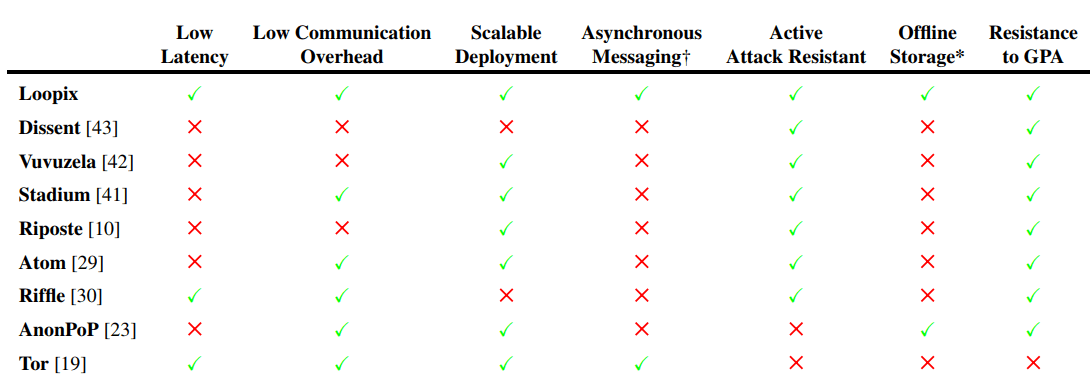
\includegraphics[width=11cm,height=11cm,keepaspectratio]{../yellowpaper/images/state-of-the-art.png}
    \caption{Comparison between anonymous communication systems}
    \label{fig:Comparison between anonymous communication systems}
\end{figure}
\hspace{-5mm}All the previous mentioned projects except VPN and dVPNs lack the economic incentive which could result in scaling issues and poor performance. Tor and I2P for example rely on donations and government funding only which covers the cost of running a node. This has discouraged volunteers to join the network and the number of routers in both networks hasn't increased much for the last few years.  Mixnets are also based on a group of volunteer agents who lack incentives to participate. Some solutions have proposed adding digital coins to messages, such that each volunteer can extract only the digital coin designated as a payment for them. However, malicious volunteers can sabotage the system by extracting and using their coins without performing their task which consists of forwarding anonymized messages since there is no verification whether the message arrives to its final destination or not. Bandwidth providers in dVPNs share their resources and are granted tokens accordingly as way of payment for their services. This is done using the blockchain technology. A good example of such technologies is Mysterium: an open source dVPN completely built upon a P2P architecture. Mysterium runs a smart contract on top of Ethereum to make sure that the VPN service is paid adequately.

\subsubsection{Scalability Layer 2 protocols}
Blockchain technology (mostly public blockchains like Bitcoin and Ethereum) suffers from a major scalability issue which is due to the fact that every node in the network needs to process every transaction, validate it and stores a copy of the entire state. The number of transactions Ethereum can process for example cannot exceed that of a single node which is currently 15 transactions per second.
\\~\\There have been multiple solutions proposed to treat the scalability issue such as sharding and off-chain computation. Both of these solutions intend to create a second layer of computation in order to reduce the load on the blockchain mainnet.
\\Off chain solutions like Plasma, Truebit and state channels process transactions outside the Blockchain while still guaranteeing a sufficient level of security and finality. State channels are better known as "payment channels". In models like the "Lightning Network", a payment channel is opened between two parties by committing a funding transaction, followed by making any number of transactions that update the channel's funds without broadcasting those to the blockchain, then closing the channel by broadcasting the final version of the settlement transaction.
\subsection{The HOPR vision}
HOPR is a decentralized incentivized mixnet that leverages privacy by design protocols. HOPR aims to protect people's metadata privacy and give them the freedom to use internet services safely and privately. HOPR runs on top of the Ethereum blockchain and uses these mechanisms to ensure users privacy via incentivisation: sphinx packet format and packet mixing, proof-of-relay and probabilistic payments.
\begin{itemize}
    \item \textit{Privacy by design:} is an approach to systems engineering and calls for privacy to be taken into account throughout the whole engineering process. HOPR believes that the Internet is a public good – a digital commons that should be safe and secure for all its users. However, it is impossible to provide such privacy using the current Internet infrastructure. What is needed is a new privacy infrastructure on top of the existing Internet. This is what HOPR has built using the sphinx packet format and packet mixing.
    \item \textit{Decentralization:} At the heart of HOPR, there is a global, decentralised network of nodes running the HOPR protocol. Decentralisation ensures that the network is independent, with no one single entity to influence its development or manipulate outcomes to their advantage. It also makes the network resilient, able to keep running even if a majority of nodes are damaged or compromised and very difficult, if not impossible, to shut down.
    \item \textit{Incentivization:} This is biggest innovation of the HOPR design. Previous privacy technologies like Tor didn't incentivize node runners to provide service which discouraged new users to join. By incentivising users, HOPR will lower the barrier to adoption. Incentivisation also encourages good behavior as the only way to earn token rewards is to behave correctly and follow the protocol.
    
\end{itemize}



 




